% !TeX encoding = utf8
% !TeX spellcheck = en_US

\section{Methods}
\subsection{Participant}
One male participant 25 years of age was recruited by the ARTORG Center for Biomedical Engineering Research. The participant was healthy and did not suffer from any known pre-existing medical conditions. This study was conducted at the Institute for Human Centered Engineering HuCE at the Bern University for Applied Sciences in Biel, Bern, Switzerland.

\subsection{Data collection}
The PPG signals were recorded with custom hardware which was designed and developed at the HuCE. The hardware consists of an ST microcontroller development board (Plan-les-Ouates, Geneva, Switzerland) and a AMS OSRAM PPG frontend (Premstätten, Styria, Austria). The PPG signal was recorded on the participant's thumb with a sampling rate $fs$ of 500\,Hz. The data was transmitted to the connected PC and was represented in real time using a  graphical user interface (GUI) programmed in Python. This GUI serves dual purposes: facilitating real-time visualization and enabling manipulation and adjustment of both the frontend and the microcontroller configurations.

\subsection{Data processing}
The PPG signals were processed in MATLAB (The MathWorks Inc., Natick, Massachusetts) Version R2023b with additional use of the signal processing and DSP system toolboxes, where finite impulse response (FIR) and infinite impulse response (IIR) filters were designed using the filter designer and afterwards applied to the signals. 

\subsection{Digital filtering}
In order to assess different filters, a IIR Chebyshev Type II and an FIR equiripple filter were chosen. The selected filters have similar pass-band and stop-band characteristics, which facilitates the comparison between the two. The stop-band characteristics can be seen in Figure \ref{fig:cheby} and \ref{fig:equiripple}. The Chebyshev Type II filter has a monotonic pass-band and an equiripple stop-band. Furthermore, it is always normalized to unity at DC and the magnitude response squared $|H(\Omega)|^2$ of the Chebyshev Type II can be computed with \cite{orfanidis_introduction_1996}
\begin{equation}
	|H(\Omega)|^2 = \frac{C_N^2\big(\frac{\Omega_{stop}}{\Omega}\big)}{C_N^2\big(\frac{\Omega_{stop}}{\Omega}\big) + \epsilon_{stop}^2},
\end{equation}
where $C_N(x)$ is the Chebyshev polynomial of degree N, which is defined by
\begin{equation}
	C_N(x) =
	\begin{cases}
		 \cos(N\cos^{-1}(x))	    	& \text{if } |x| \le 1 \\
		\cosh(N\cosh^{-1}(x)),		& \text{if } |x| > 1.
	\end{cases}
\end{equation} 

\begin{table}% Half width table
	\caption{Used filters applied to the signal.}
	\centering % Horizontally center the table
	\begin{tabularx}{\linewidth}{l|l|X|} % Manually specify column alignments with L{}, R{} or C{} and widths as a fixed amount, usually as a proportion of \linewidth
		\toprule
		Filter & Filter type & Order\\
		\midrule
		Chebyshev Type II & IIR Lowpass & 10 \\
		Equiripple  & FIR Lowpass & 211 \\
		\bottomrule
	\end{tabularx}
	\label{tab:packages}
\end{table} 

The principal limitation of designing FIR filters using the window method is the inability to modulate the approximation error across varying frequency ranges. Therefore, it is frequently advantageous to utilize the minimax strategy, which minimizes the peak error, or to apply an error criterion incorporating frequency weighting in filter design. This methodology produces the most optimal filter achievable for a specified set of requirements. So that a FIR filter with minimum effort can be designed the FIR Equiripple method is used. \cite{noauthor_introduction_nodate} 

In order to design an equiripple filter from a set of frequency domain specifications, the weighted error model is used, where $\epsilon(\hat{\omega})$ is 
\begin{equation}
	\epsilon(\hat{\omega}) = W(\hat{\omega}) |H_d(e^{j\hat{\omega}}) - H(e^{j\hat{\omega}})|,
\end{equation}
where the weighted error is defined in terms of a non-negative error weight $W(\hat{\omega}) \ge 0$ and the difference between the \emph{desired} $H_d(e^{j\hat{\omega}})$ and \emph{realized} $ H(e^{j\hat{\omega}})$ filter's base-band frequency response. 
Equiripple FIR filters satisfy the \emph{minimax error criterion}, which asserts that the optimal solution is achieved when $\delta = \min(\max(|\epsilon(\hat{\omega})|))$, with $\hat{\omega} \in [0, \hat{\omega}_s/2]$, where $\delta$ is called the \emph{minimax error} or \emph{external error}.  \cite{williams_electronic_2006}

The band-pass and band-stop frequencies were set to 8\,Hz and 14\,Hz, respectively with a stop-band attenuation of 80\,dB. Both filters were implemented as fixed point arithmetic on the microcontroller, which then applied the filters during the recording of the signal.

\begin{figure}[H]
	\centering
	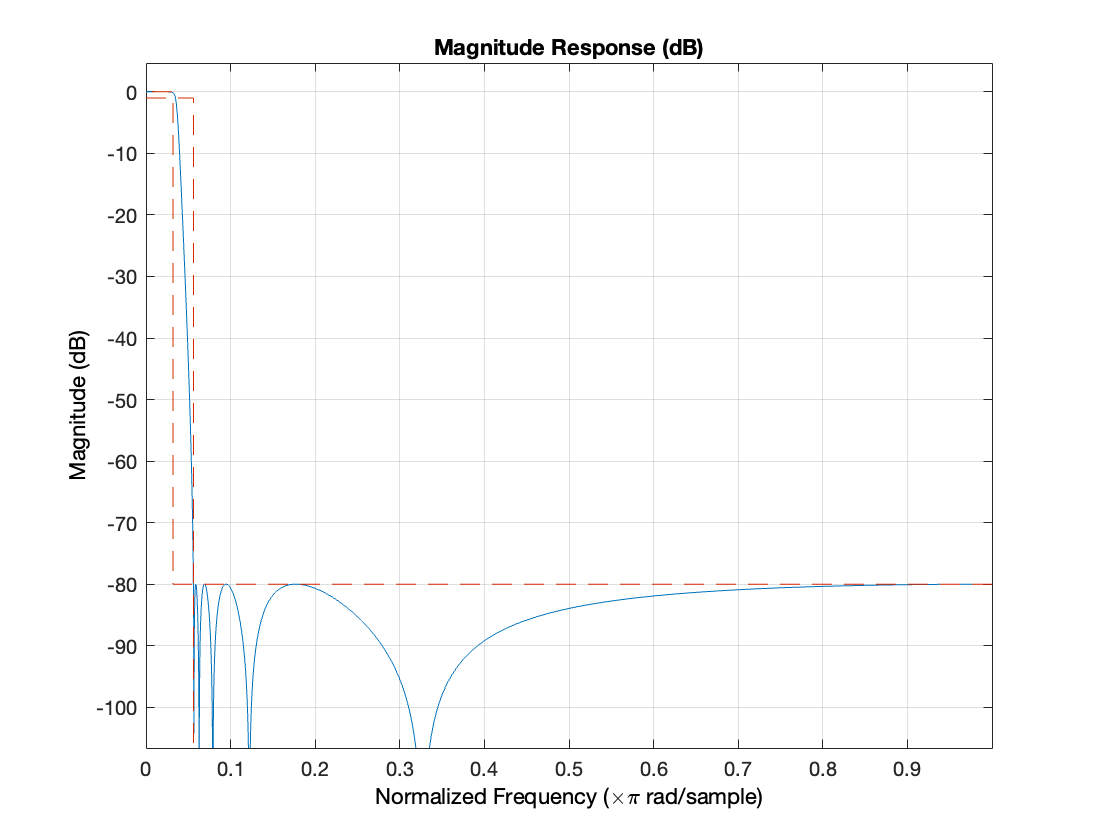
\includegraphics[width=\linewidth, trim={2.5cm, 1cm, 4cm, 1cm}, clip]{Figures/chebyII.png}
	\caption{Frequency response of IIR Chebyshev Type II.}
	\label{fig:cheby}
\end{figure}

\begin{figure}[H]
	\centering
	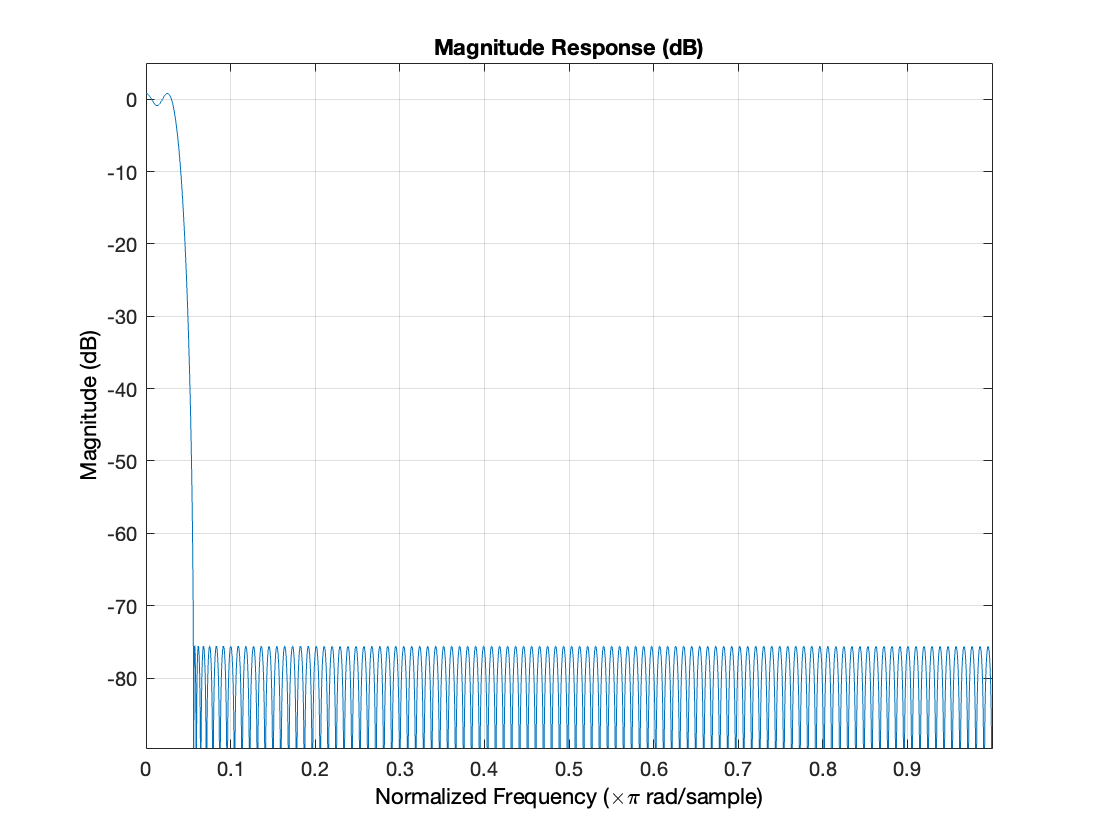
\includegraphics[width=\linewidth, trim={2.5cm, 1cm, 4cm, 1cm}, clip]{Figures/equiripple.png}
	\caption{Frequency response of FIR Equiripple.}
	\label{fig:equiripple}
\end{figure}


\subsection{Filter performance evaluation}
So that both filters could be compared objectively their power spectral denstity was computed. The discrete-time Fourier transform of a random signal's autocorrelation function $R_{xx}(k)$ is defined as its power spectrum $S_{xx}(\omega)$. The frequency content of the random signal $x(n)$ is represented by the power spectrum 
\begin{equation}
	S_{xx}(\omega) = \sum_{-\infty}^{\infty} R_{xx}(k)\cdot e^{-j\omega k},
\end{equation}
where $\omega = 2\pi f/f_s$ is the digital or normalized frequency in radians per sample.

Furthermore, the quantity $S_{xx}(f)/f_s$ represents the power per unit frequency interval, which describes the \emph{power spectrum} or \emph{power spectrum density}. It shows how the signal's power is spread out among the individual frequencies. \cite{orfanidis_introduction_1996}

The mentioned filters should have a large amount of their power in the pass-band region and much of the power in the stop-band region should be absent, so that the high frequency noise is attenuated. This observation is corroborated by an objective visual inspection of the power spectra of both filters. The power spectral density plots of both filters can be seen in Figure \ref{fig:powerspectra}.

\begin{figure}
	\centering
	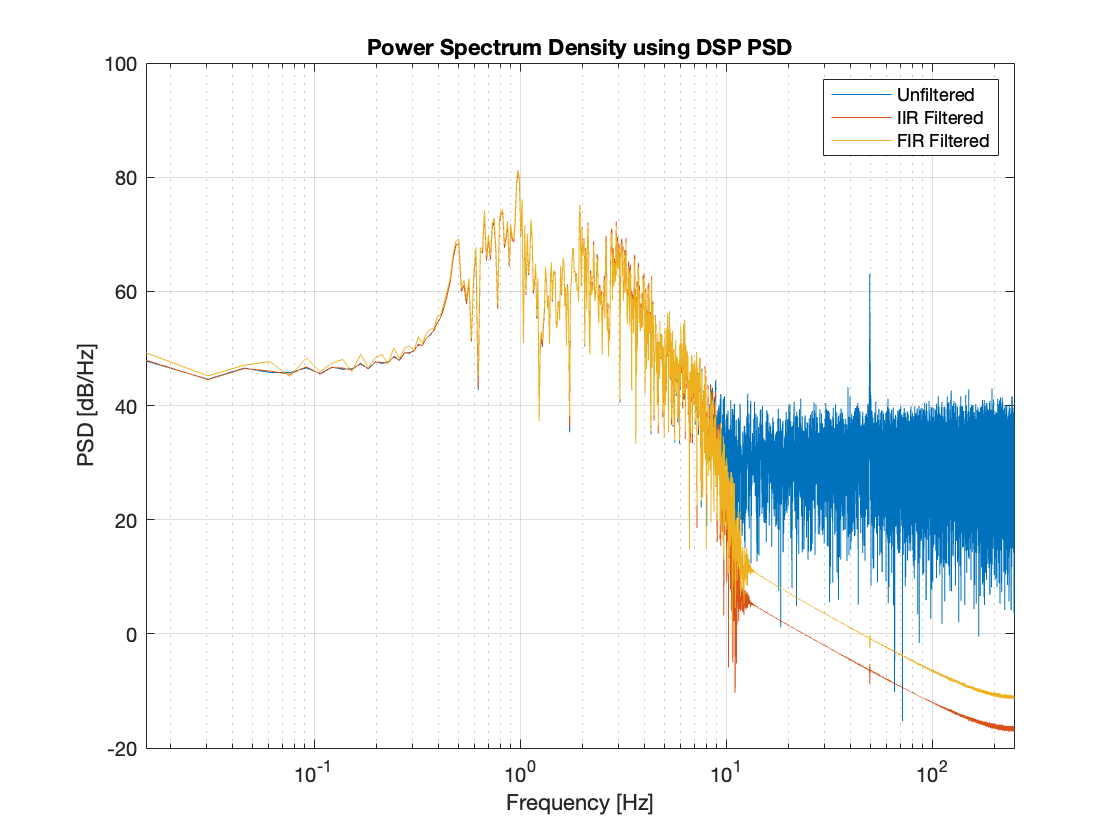
\includegraphics[width=\linewidth, trim={2.5cm, 1cm, 2cm, 1cm}, clip]{Figures/powerspectra.png}
	\caption{Power spectrum of the IIR Chebyshev Type II and FIR Equiripple filter compared to the unfiltered power spectrum.}
	\label{fig:powerspectra}
\end{figure}


\subsection{Heartbeat peak detection}
In order to detect peaks of the heartbeat signals, the derivative of the signal was needed and was computed via a simple algorithm based on a backward implicit finite difference method, as depicted in Equation \eqref{eq:finite_diff}
\begin{equation}\label{eq:finite_diff}
	u'(x) = \frac{u(x) - u(x-h)}{h},
\end{equation}
where $u(x)$ is the value of the current time sample, $u(x-h)$ is the value of the previous time sample two samples ago and $h$ is the distance between each time sample, which was $1/fs$. 

To classify a peak, the following criteria were employed: the signal had to reach a threshold value equaling 40\% of the maximum signal value, and the derivative of the signal needed to lie within $\pm5\%$ of the maximum and minimum derivative values. To prevent multiple detections within a short interval, a waiting period of 200 samples was enforced. If these conditions were met, the index was classified as a peak. Given the above conditions, if the PPG signal values were to decrease significantly, subsequent peaks might fail to be detected. To correct for this potential issue, the peak threshold was reset after a duration of $2f_s$, establishing a new threshold based on the current maximum value. The algorithm was evaluated through visual inspection of the marked peaks. An interval of 10 seconds can be seen in Figure \ref{fig:peaks}.
\begin{figure}
\centering
	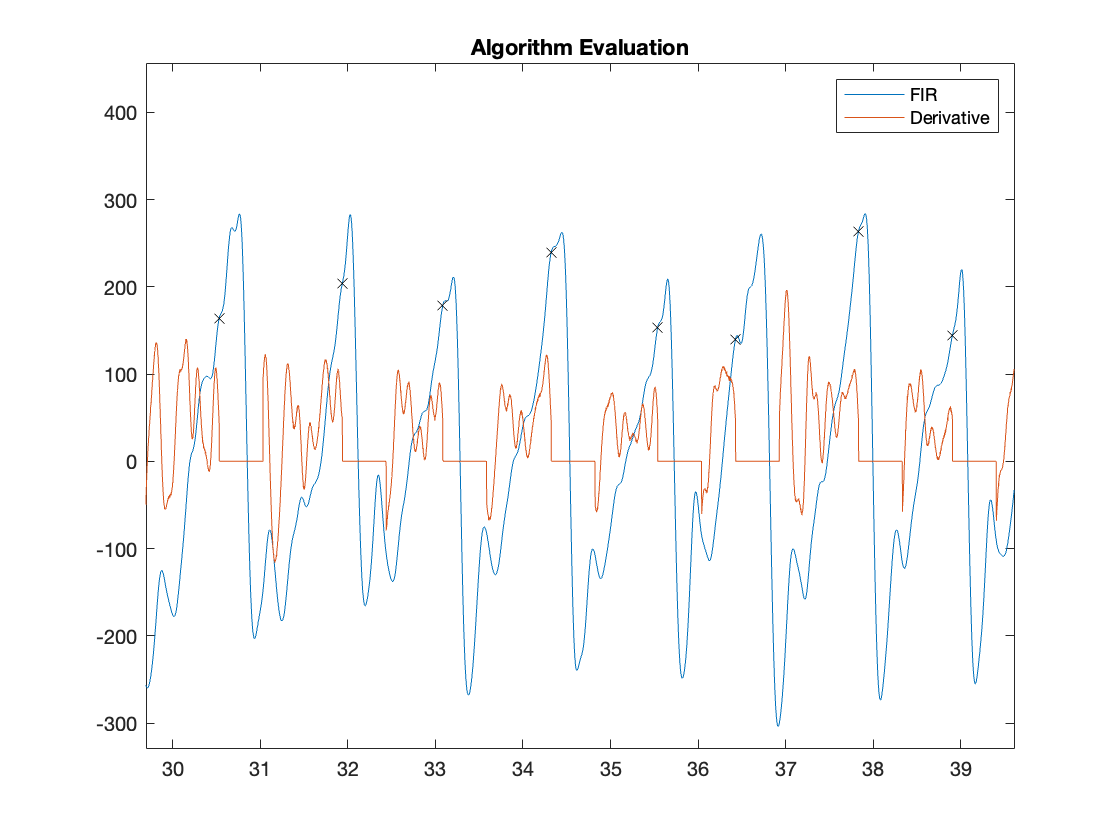
\includegraphics[width=\linewidth, trim={2.5cm, 1cm, 2cm, 1cm}, clip]{Figures/peaks.png}
	\caption{Evaluation of the heartbeat peak detection algorithm.}
	\label{fig:peaks}
\end{figure}
In order to evaluate the algorithm the peaks were counted manually and then compared to the number of peaks detected by it. The evaluation of the MATLAB implementation can be found in the results.

\subsection{Heart rate calculation}
The heart rate was computed during intervals of $15f_s$, where the number of peaks was divided by the number of intervals and then multiplied by $60$ in order to compute the heart rate in [beats per minute].

\subsection{Microcontroller porting}
After the peak detection algorithm was tested in MATLAB, the algorithm was programmed in C and ported onto the microcontroller. 

\subsection{Sensitivity of peak detection algorithm}
In order to get some sort of a metric to describe the performance of the implemented heartbeat peak detection algorithm, the sensitivity was calculated using Equation \eqref{eqn:accuracyEquation}

\begin{equation}
	\label{eqn:accuracyEquation}
	\text{Sensitivity} = \frac{TP}{TP+FN} \times 100 \%.
\end{equation}

where $TP$ is the number of true positives (i.e. the algorithm correctly identified a heartbeat peak) and $FN$ is the number of false negatives (i.e. the algorithm was unable to identify a heartbeat peak) \cite{trevethan_sensitivity_2017}.












